%!TEX root = ../template.tex
%%%%%%%%%%%%%%%%%%%%%%%%%%%%%%%%%%%%%%%%%%%%%%%%%%%%%%%%%%%%%%%%%%%
%% chapter1.tex
%% NOVA thesis document file
%%
%% Chapter with introduciton
%%%%%%%%%%%%%%%%%%%%%%%%%%%%%%%%%%%%%%%%%%%%%%%%%%%%%%%%%%%%%%%%%%%
\chapter{Experimental Observations and Validations}
\label{cha:experimentalEvaluation}

In this chapter we describe the work we conducted for the validation and evaluation of our proposed in-memory TREDIS solution, detailed in \ref{cha:implementation}. We will mostly evaluate the impact of the biggest and most important components, such as the \gls{kvs} layer and the Proxy, while also analysing the impact of the attestation component. However, as for the component responsable for the authentication of the clients, we consider it to be out of the scope of our study.

Here, we start by presenting the metrics we intend to evaluate, along with the test benches we defined to test our prototype.
We then go deeper about each test bench, describing the results obtained during the experimental evaluation of each one of those scenarios, leading to a discussion later in this chapter aiming to compare those results and, finally, ending with a summary of the chapter.


\section{Criteria for Experimental Observations}
\label{sec:criteriaForExperimentalObservations}

Our evaluation process is simple: track our TREDIS solution's behavior through all the different configurations, incrementally adding more layers to the system. Thus, we intend to evaluate our TREDIS solution on each possible configuration, starting with a basic model and slowly add more components to the system, while also making experimental observations about the impact they have. 

During the evaluation process we focus on measuring: 1) the performance impact each component has in the system while running with or without \gls{sgx}, through a latency and throughput analysis, and 2) resource allocation during runtime, including memory and CPU usage. 

There are other particular measurements that we found useful to introduce, that we detail later, while describing the test benches individually.
Adding to that, we also analyse the system's behavior under different client-workloads, by scaling up the number of requests and varying the typology of requests made to the system.


\section{Deployment of Testbench Environments}
\label{sec:testBenchEnvironments}

As said before, we intend to evaluate our in-memory TREDIS system behavior by incrementally adding components to it, which will add security to the whole system, and see what impact they have on it. In order to do that, we define a list of Testbench (TB) scenarios to help us evaluate the system gradually.

First, our idea is to benchmark the \gls{kvs} Redis layer running normally inside our cloud server, to use it as a reference point to what is the expected behavior of a in-memory Redis \gls{kvs} is in our server. For that, we define the Testbench 1 (TB1) as a default version of Redis, with TLS support, running in our OVH cloud server.

As the next step, we analyze the impact that \gls{sgx} has in a \gls{sgx}-enabled Redis. For that we define TB2 as our cloud server running the Redis \gls{kvs} component inside a SGX-enabled SCONE container.

TB3 assumes the addition of the Proxy component to the solution, in order to benchmark its impact on the system. Thus, we define TB3 as a Redis component running inside a SGX-enabled SCONE container, along with a Single Proxy instance.

In TB4, we deploy the Proxy component on top of \gls{sgx}, resulting on benchmarking a system composed by a Redis \gls{kvs} running inside a SGX-enabled SCONE container, along with a Single Proxy instance also running inside \gls{sgx}.

For TB5, we added the attestation property to the components, used to assure that they run in private memory regions on top of \gls{sgx} and that they are only executed by the right enclave. Here we measure the impact it has to attestate each component upon start.

With all the system model defined in \ref{cha:systemModel_and_design} in place, we define two more test benches TB6 and TB7 to evaluate the whole system's behavior against different client request overloads (increased number of requests plus different size payloads) and against different typologies of requests (i.e., 10\% Writes : 90\% Reads), respectively.

This are the testbench scenarios we follow in order to evaluate our solution while running the Redis layer in all the three configurations we detailed in previous chapters: Standalone Redis, Master-Slave Redis and Clustered Redis.


\section{Observations with Cloud-based Standalone REDIS}
\label{sec:cloudS_Redis}

In this section, we analize our solution running the in-memory Redis component configured as a single instance \gls{kvs}. The experimental evaluation will be done following the test benches defined above, to access the impact of \gls{sgx} in our system, analysing both the performance and resource allocation impact that each secured component has in the system.

As we detailed in \ref{sec:implementationArchitecture}, we run our solution on a cloud system with \gls{sgx}-enabled hardware, while our client benchmark applications run on a local machine with commodity hardware, in order to simulate a real-world use-case where the network has a major impact in the performance of a system.

\subsection{Latency Impact of SGX-Enabled REDIS}

To study and compare the latency levels of TREDIS with and without \gls{sgx}, we evaluate our solution by complying to the testbench TB1, TB2, TB3 and TB4 (see \ref{sec:testBenchEnvironments} for details) definitions, with network conditions of $\approx$116Mb/s Download and $\approx$114Mb/s Upload speed. It is important to mention that, for the first two testbenches in which our client application point directly to the Redis \gls{kvs} layer, we used redis-benchmark to make the requests and benchmark the solution. However, with the addition of the Proxy layer in TB3, we had to switch to a HTTP-enabled client, Jmeter.

Thus, we start to benchmark our solution according to TB1, which results on an average 33,97 millisecond response time that we can use as a base value.
By comparing it to the value of TB2, we note that the addition of \gls{sgx} security properties to the \gls{kvs} component induced a latency penalty of 4,89\%, as we can see in Table \ref{table:latencySingleRedis}. This value is expected since, as we studied in previous chapters, \gls{sgx} induces in performance overheads caused by the time spent dealing with heavy functions and mechanisms in order to keep the integrity and confidentiality of the data.

\begin{table}[ht]
	\caption{Latency impact of SGX in Standalone Redis} % title of Table
	\centering % used for centering table
	\begin{tabular}{c c} % centered columns (4 columns)
		\hline\hline %inserts double horizontal lines
		\textbf{Configuration} & \textbf{Latency} \\ [0.5ex] % inserts table
		%heading
		\hline
		Redis & 33,97ms\\
		\hline
		SGX-enabled Redis & 35,63ms \\
		\hline
	    SGX-enabled Redis + Proxy & 37,3ms \\
		\hline % inserts single horizontal line
	    SGX-enabled Redis + SGX-enabled Proxy & 44ms\\ [1ex] % [1ex] adds vertical space
		\hline %inserts single line
	\end{tabular}
	\label{table:latencySingleRedis} % is used to refer this table in the text
\end{table}

As we detailed before in previous chapters, our TREDIS solution includes a Proxy component that also adds overhead to the system, and it is expected to add even more when running inside \gls{sgx}. For that analysis, we run TB3 and TB4, in order to evaluate Proxy's impact in the overall system. With the addition of this component, we observe an additional 4,69\% overhead compared to TB2. This value is something we can deal with due to the utility we give to this component in particular. However, the 17,96\% latency increase that \gls{sgx} imposes to the Proxy component can lead to a subjective conclusion. This overhead is covered by the \gls{sgx} impact, but also by it being a more I/O-intensive component, thus resulting on a higher probability of making system calls.

\subsection{Generic Throughput Observation}

In order to measure the impact that enabling \gls{sgx} has on the throughput of our solution, we follow the same test benches as the ones used in the latency test - TB1, TB2, TB3 and TB4. Our following evaluation is based on the average measurements of a set of identical tests, each one consisting on one client making 10 000 requests with 10 Bytes worth of data over the network.

\begin{figure}[htbp]
	\centering
	{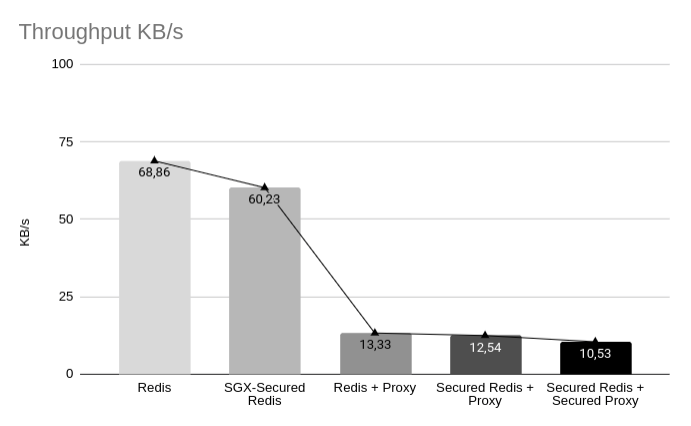
\includegraphics[width=0.7\linewidth]{graphThroughputStandalone}}
	\caption{Throughput impact of SGX in Standalone Redis}
	\label{fig:graphThroughputStandalone}
\end{figure}

Here, the addition of \gls{sgx} to the Redis component induces in a 12,53\% overhead, that we observe in Figure \ref{fig:graphThroughputStandalone} in the tests made via redis-benchmark, in which the client application connects directly with the \gls{kvs} layer itself, via TCP. 

However, in TB3 and TB4 results, we can see that adding the Proxy component to the system drops significantly the solution's throughput levels. This is expected since the requests start to be done via HTTP, which induces in losses of $\approx$80\% compared to TCP. With the requests being now done to the Proxy, we observe only a 5,93\% throughput penalty on running the \gls{kvs} on top of \gls{sgx}, that we can note in Table \ref{table:throughputSingleRedis}, along with a 16,02\% drop when enabling the Proxy layer to also execute on top of \gls{sgx}. The reasons are related to the performance overheads know to be induced by \gls{sgx} itself. Note that the Proxy component is an application written in Java, making the inclusion of JVM and other java libraries fundamental, thus the image running in the SCONE container on top of \gls{sgx} is heavier, resulting on to having to leave some Java code outside the enclave.


\begin{table}[ht]
	\caption{Proxy impact in Standalone Redis} % title of Table
	\centering % used for centering table
	\begin{tabular}{c c} % centered columns (4 columns)
		\hline\hline %inserts double horizontal lines
		\textbf{Configuration} & \textbf{Throughput} \\ [0.5ex] % inserts table
		%heading
		\hline
		Redis + Proxy & 13,33KB/s\\
		\hline
		SGX-enabled Redis + Proxy & 12,54KB/s \\
		\hline % inserts single horizontal line
		SGX-enabled Redis + SGX-enabled Proxy & 10,53KB/s\\ [1ex] % [1ex] adds vertical space
		\hline %inserts single line
	\end{tabular}
	\label{table:throughputSingleRedis} % is used to refer this table in the text
\end{table}



\subsection{Evaluation of Specific Benchmarks and Operations}
\label{ssec:specificBenchmarksRedisS}

As a way to evaluate our solution's behavior facing more specific benchmarks, we test it by following the TB6 and TB7. 

Here we present how different operation ratios influence the system throughput. By looking at Figure \ref{fig:thptDiffCombinationsSingleRedis}, we can see that the results on how TREDIS handles these different combinations of requests with small payloads do not vary much. This absence of difference might be related to Redis high performance levels, specially with small payloads, where it takes almost no time to compute. Therefore the numbers should look alike as they do.  

\begin{figure}[htbp]
	\centering
	{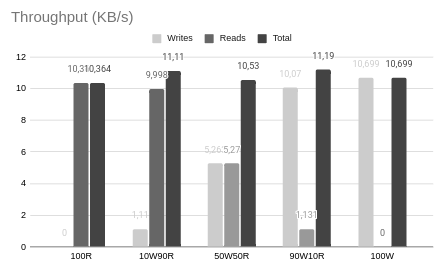
\includegraphics[width=0.6\linewidth]{thptDiffCombinationsSingleRedis}}
	\caption{Throughput with different sets of operations}
	\label{fig:thptDiffCombinationsSingleRedis}
\end{figure}

However, with the increase of payload size, we start to see significant drops in the number of operations done, along with higher response times, as we can see in the Table \ref{table:throughputPayloads}. This is due to the Redis-server not handling big payloads very well, since it is mostly single-threaded, thus needing more time to handle requests.

\begin{table}[ht]
	\caption{Throughput values with different size payloads} % title of Table
	\centering % used for centering table
	\begin{tabular}{c c c c} % centered columns (4 columns)
		\hline\hline %inserts double horizontal lines
		\textbf{Payload Size} & \textbf{Operations p/sec} & \textbf{Latency}\\ [0.5ex] % inserts table
		%heading
		\hline
		10B & $\approx$22 & $\approx$44ms\\
		\hline
		10KB & $\approx$20 & $\approx$46ms\\
		\hline % inserts single horizontal line
		100KB & $\approx$12 & $\approx$59ms\\ [1ex] % [1ex] adds vertical space
		\hline %inserts single line
	\end{tabular}
	\label{table:throughputPayloads} % is used to refer this table in the text
\end{table} 

Also, to comply with TB6, we scale the number of requests made to the server, in order to see differences in the behavior of the system. However, we find it hard to simulate \gls{epc} memory page swapping with small payloads, as it takes a long time to reach near the \gls{epc} memory size, so we increase the payloads to 100 KBytes. By doing that, we encounter an unexpected problem: when reaching the maximum RSS size defined for Redis upon start (default is 64 MBytes), the container crashes. We later found out that this problem is targeted in SCONE's website\footnote{https://sconedocs.github.io/faq/}, where they explain it to happen due to the SGX version (SGX v1) we are using not supporting dynamic allocation of memory, thus \textit{"enclaves must allocate all memory at startup since enclaves are fixed"}. This causes the memory usage of Redis to be higher than it needs to be, since to prevent it from crashing we need to allocate memory upon start that we do not know we will need, leading to larger startup times. However, SCONE also affirms that the next version of SGX (SGX v2) will support dynamic allocation, which tackles this problem. 


\subsection{Standalone REDIS System Resources}
\label{ssec:SingleRedis_MemCPU}

Here we evaluate our solution's memory consumption and CPU usage during runtime. 
For the purpose of this test, our client application made requests to the Proxy during 180 seconds with 1 KBytes worth of data.  

In the graphs we present in Figure \ref{fig:MemoryConsumption_standalone}, we observe some changes in the system when running it on top of \gls{sgx} and outside of it. First of all, we notice that the dataset size increases faster if running without \gls{sgx} support, since the system is faster and its throughput levels are higher, resulting in more operations made over the dataset in the same time period. We can also see that the Resident Set Size (RSS) in one case is dynamic, while in the other is static. This calls back to what we stated in the section before, where we mentioned that SGX v1 does not support dynamic allocation of memory, thus only relying on the memory size specified upon creation which remains static throughout execution. In Figure \ref{fig:SgxStandaloneMemory} we see just that, a static RSS value during the entire evaluation. Note that this RSS value defines the memory available for a Redis instance to scale during its execution. Thus, running Redis inside SGX might induce into memory problems if using SGX v1, since either the system reaches the point where it is left with no memory available to run and stops, or it is created with huge amounts of memory, which might not be necessary, inducing it to big startup times since it needs to allocate more memory upfront.

\begin{figure}[htbp]
	\centering
	\subbottom[) no SGX]{%
		\label{fig:noSgxStandaloneMemory}
		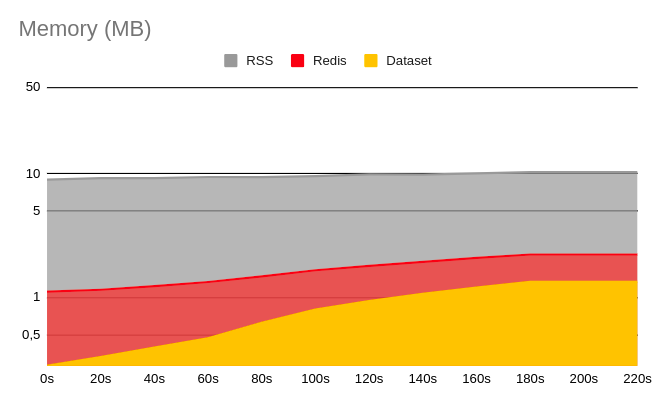
\includegraphics[width=0.45\linewidth]{memoryRedisNoSGX_standalone}}%
	\subbottom[) with SGX]{
		\label{fig:SgxStandaloneMemory}
		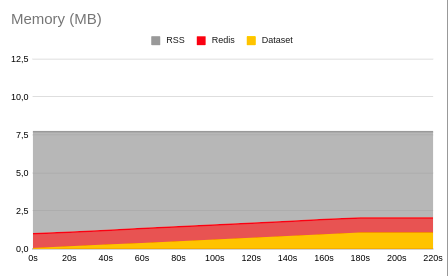
\includegraphics[width=0.45\linewidth]{memoryRedisSGX_standalone}}
	\caption{Standalone Redis memory consumption during runtime}
	\label{fig:MemoryConsumption_standalone}
\end{figure}

As for the CPU usage, we show in Figure \ref{fig:cpuUsageStandalone} the impact that \gls{sgx} has. On the left, we see the CPU resources that go into the execution of the solution without this extra layer of security, remaining near 0\% for Redis while the Proxy shows values of around 5-8\%, due to all I/O operations it handles. On the right, we see more expressive results, where the addition of \gls{sgx} results on higher CPU usage, specially by the Proxy component, due to its size causing it not to fit entirely inside the \gls{epc}. However, since this test also induces in a high density of requests, we do not consider this behavior to be unexpected.

\begin{figure}[htbp]
	\centering
	\subbottom[) no SGX]{%
		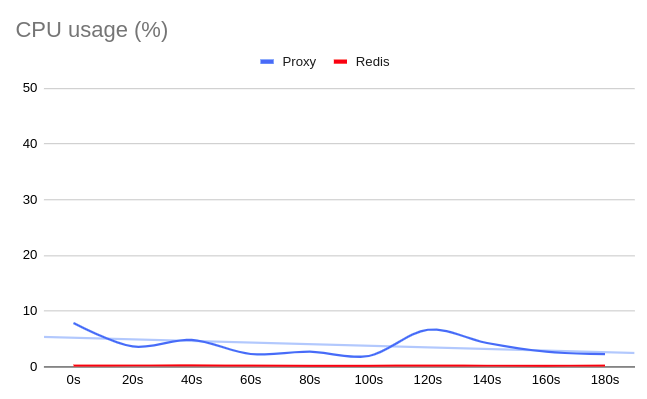
\includegraphics[width=0.5\linewidth]{cpuUsageStandalone_noSGX}}%
	\subbottom[) with SGX]{
		\label{fig:sgxCPUusage_standalone}
		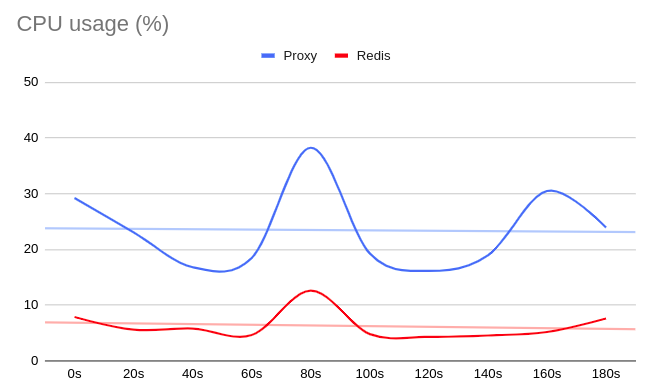
\includegraphics[width=0.5\linewidth]{cpuUsageStandalone}}
	\caption{Standalone Redis CPU usage during runtime}
	\label{fig:cpuUsageStandalone}
\end{figure}

\section{Observations with Cloud-based Master-Slave REDIS}
\label{sec:cloud_MS_Redis}

Here we present our observations while testing our solution with the Redis layer in a Master-Slave configuration. We run the \gls{kvs} with three replicas, one being a master node, and the other two being read-only slave nodes. 

Hereupon, this experimental evaluation follows the same test benches that we used in Section \ref{sec:cloudS_Redis}, to analyze the impact that enabling \gls{sgx} support to our components has in the whole solution.

We run the test scenarios in the same environment previously used, in a cloud system with \gls{sgx} support, while making the requests in a local machine over the network, with the network speed being of $\approx$117Mb/s Download and $\approx$119Mb/s Upload.


\subsection{Latency Impact of SGX-Enabled Master-Slave REDIS}

In order to evaluate the latency impact of \gls{sgx} in our solution, as we just mentioned, we intend to execute the TB1, TB2, TB3 and TB4 scenarios, incrementally adding components to the system, while enabling \gls{sgx} support to each one of them along the way. 

We start the test by making requests to the server with redis-benchmark as the client application when communicating directly to the Redis-server, and then switching to Jmeter to communicate through HTTP with the Proxy component.

\begin{table}[ht]
	\caption{Latency impact of SGX in M-S Redis} % title of Table
	\centering % used for centering table
	\begin{tabular}{c c} % centered columns (4 columns)
		\hline\hline %inserts double horizontal lines
		\textbf{Configuration} & \textbf{Latency} \\ [0.5ex] % inserts table
		%heading
		\hline
		Redis & 32,48ms\\
		\hline
		SGX-enabled Redis & 32,97ms \\
		\hline
		SGX-enabled Redis + Proxy & 34,45ms \\
		\hline % inserts single horizontal line
		SGX-enabled Redis + SGX-enabled Proxy & 41,3ms\\ [1ex] % [1ex] adds vertical space
		\hline %inserts single line
	\end{tabular}
	\label{table:latencyMasterSlaveRedis} % is used to refer this table in the text
\end{table}

In Table \ref{table:latencyMasterSlaveRedis} we can observe a similar behavior compared to the values we saw for our solution running a single instance Redis, as the latency time increases with the components and extra security we add to the system. Here we can see a 1,5\% drop with the inclusion of \gls{sgx} support to the \gls{kvs} layer. Connecting the Proxy, however, costs the system around 4,3\%, and protecting it with \gls{sgx} induces in a 16,6\% latency drop, again originated from the fact that it is a I/O-intensive component, which lead to more system calls being done by it while inside the enclave, which by \gls{sgx}' definition is a major influencer in performance dropping. Adding to that, it is a Java application, resulting in a bigger image which can lead to some of the code having to be placed outside the enclave.

\subsection{Generic Throughput Comparative Observations}
For our throughput evaluation we use the same configuration as we did for Standalone Redis, consisting in one client thread doing all the 10 000 requests with a payload of 10 Bytes, while registering the average results of multiple tests.

\begin{figure}[htbp]
	\centering
	{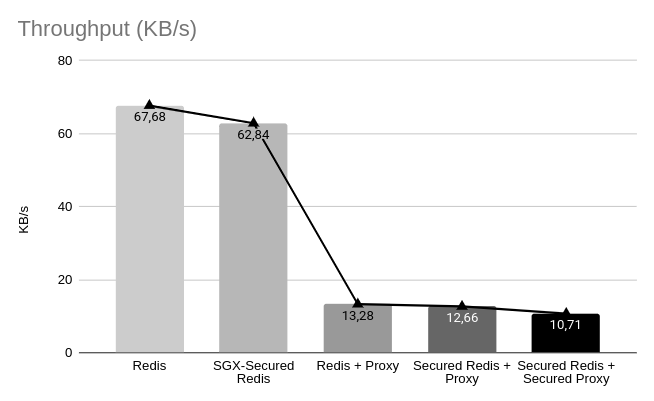
\includegraphics[width=0.65\linewidth]{graphThroughputMasterSlave}}
	\caption{Throughput impact of SGX in M-S Redis}
	\label{fig:graphTroughputMasterSlave}
\end{figure}

In Figure \ref{fig:graphTroughputMasterSlave} we can observe a 7,15\% drop by securing the \gls{kvs} layer with \gls{sgx}, which is a slightly smaller loss than the one we observed in the Standalone tests. However, we observe once again a considerable penalty with the addition of the Proxy layer, which along with the switch from TCP requests to HTTP requests causes a huge throughtput drop of around 80\%, even without any \gls{sgx} inclusion. With the inclusion of this extra layer of security, our solution exhibits a loss of 15,45\%.



\subsection{Throughput with Specific Benchmarks and Operations}

Here we test the behavior of our Master-Slave configured solution against different operation ratios and different payload sizes. 
In Figure \ref{fig:thptDiffCombinationsMasterSlaveRedis} we can see pretty much the same results we had with Redis running in Standalone mode, either while running 100\% writes, or 100\% reads, or any other combinations we present here.  

\begin{figure}[htbp]
	\centering
	{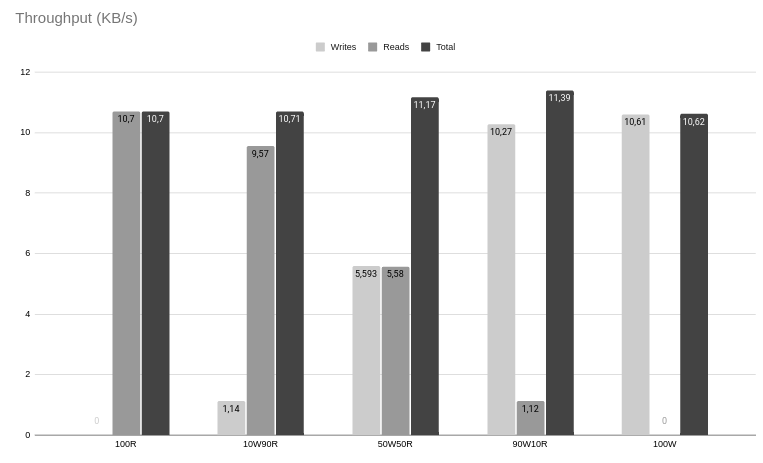
\includegraphics[width=0.7\linewidth]{thptDiffCombinationsMasterSlaveRedis}}
	\caption{Throughput with different combinations of operations}
	\label{fig:thptDiffCombinationsMasterSlaveRedis}
\end{figure}

In the evaluation regarding the increment of the payload of the requests, shown in Table \ref{table:throughputPayloadsMS}, we observe a similar behavior as we did with Redis Standalone, where bigger payloads lead to less performance. However, with a Master-Slave configuration we got slightly higher results while working with smaller size payloads.

\begin{table}[ht]
	\caption{Throughput differences with different size payloads} % title of Table
	\centering % used for centering table
	\begin{tabular}{c c c} % centered columns (4 columns)
		\hline\hline %inserts double horizontal lines
		\textbf{Payload Size} & \textbf{Operations p/sec} & \textbf{Latency}\\ [0.5ex] % inserts table
		%heading
		\hline
		10B & $\approx$23 & $\approx$42\\
		\hline
		10KB & $\approx$21 & $\approx$43\\
		\hline % inserts single horizontal line
		100KB & $\approx$12 & $\approx$56\\ [1ex] % [1ex] adds vertical space
		\hline %inserts single line
	\end{tabular}
	\label{table:throughputPayloadsMS} % is used to refer this table in the text
\end{table} 

This slight increase compared to Standalone mode is induced by the replication given by the Master-Slave model, in which all replicas are available to handle read operations, thus making the impact that those kind of operations have on the system way lower.   


\subsection{Master-Slave REDIS System Resources}
\label{ssec:MSRedis_MemCPU}

To perform a system resources evaluation during our solution's runtime, we set our client to make requests with 1 KBytes to the system for a total of 180 seconds.  

The graphs we present in Figure \ref{fig:noSgxMemoryConsumption} and \ref{fig:sgxMemoryConsumption} show exactly how the server manages the memory of our Redis layer, either with or without the \gls{sgx} security properties. 
In the first one, we can observe the behavior of both the master node and the slave nodes, in which we see a slightly faster memory increase on the master, since it is the only replica responsible to perform writes in the \gls{kvs} in this configuration. Thus the master receives the data first, whereas the slaves have to wait for the replication to happen, in order to update their own dataset. 
They behave similarly throughout the execution of the test, achieving eventual consistency by the end, thus ending the test with same exact dataset. 

\begin{figure}[htbp]
	\centering
	\subbottom[) master node]{%
		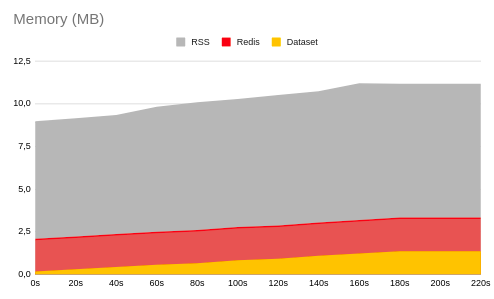
\includegraphics[width=0.4\linewidth]{memoryRedisNoSGX}}%
	\subbottom[) slave node]{
		\label{fig:noSgxSlaveMemory}
		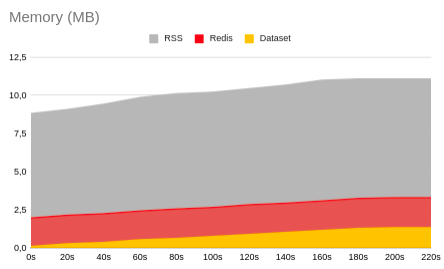
\includegraphics[width=0.4\linewidth]{memoryRedisNoSGX_slave}}
	\caption{M-S Redis memory consumption}
	\label{fig:noSgxMemoryConsumption}
\end{figure}

\begin{figure}[htbp]
	\centering
	\subbottom[) master node]{%
		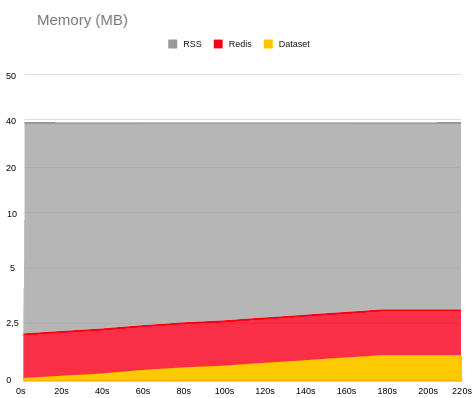
\includegraphics[width=0.4\linewidth]{memoryRedisSGXMS}}%
	\subbottom[) slave node]{
		\label{fig:sgxSlaveMemory}
		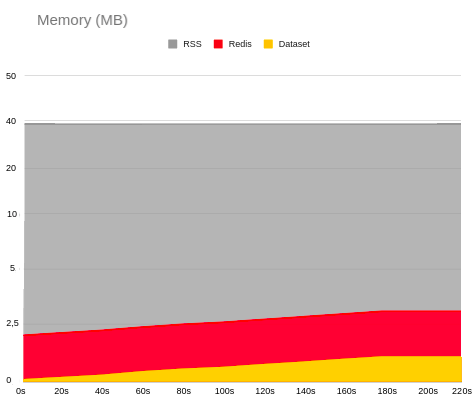
\includegraphics[width=0.4\linewidth]{memoryRedisSGXMS_slave}}
	\caption{SGX-enabled M-S Redis memory consumption}
	\label{fig:sgxMemoryConsumption}
\end{figure}

Note that without \gls{sgx} support, the memory allocated to run the Redis layer (shown as grey in the graphs - RSS) follows dynamically both the rise of the Dataset size and the Redis instance size. This means that, without \gls{sgx}, this layer can allocate memory on-demand, optimizing its memory consumption during runtime. However, as we have mentioned before, the same does not happen for \gls{sgx}-enabled components, since SGX version v1 does not include this dynamic allocation of memory, thus failing to scale the application's memory size, while running inside the enclave. This is why we see a static RSS value in both graphs presented in Figure \ref{fig:sgxMemoryConsumption}. Besides that, the values shown are similar to the ones shown in the Standalone evaluation, as the Dataset memory size increases gradually alongside the Redis memory size. 

The memory consumption values we show in the figure covering the \gls{sgx}-enabled solution are lower at the end of the 180 second test, which is expectable since the throughput numbers are inferior, therefore less writes are made in that same period of time. And also, just to mention that in Figures \ref{fig:noSgxMemoryConsumption} and \ref{fig:sgxMemoryConsumption} we only show graphs for one slave node because they both have a similar behavior throughout the tests, since they both replicate the same master instance.

For the CPU, we can see what resources go into the execution of the tests in Figure \ref{fig:cpuUsageMS}, where we notice once again almost 0\% CPU usage when dealing with a Redis \gls{kvs} without \gls{sgx}, whereas if we enable \gls{sgx} support, this value rises to $\approx$8\%, in which the master node shows to be the one node needing more resources, due to being in charge of replicating the data to all the slave nodes in the system.

As for the Proxy impact in the CPU, we can see a similar behavior to what we observed with Standalone Redis, since not much have changed for this component. We see the same $\approx$8 to 10\% when running without \gls{sgx} security properties, while more expressive results when executed on top of \gls{sgx}.

\begin{figure}[htbp]
	\centering
	\subbottom[) no SGX]{%
		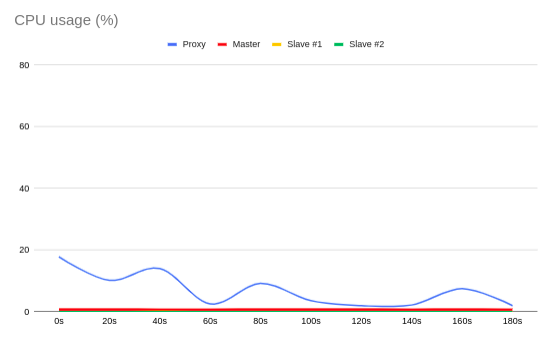
\includegraphics[width=0.51\linewidth]{cpuUsageMasterSlave_noSGX}}%
	\subbottom[) with SGX]{
		\label{fig:sgxCPUusage}
		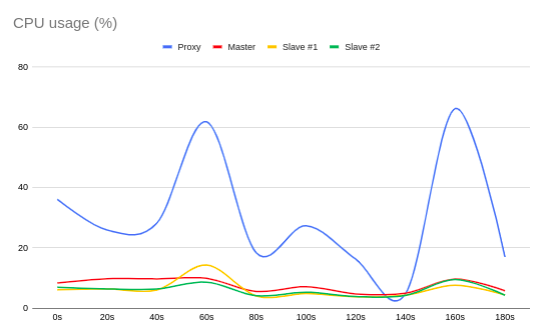
\includegraphics[width=0.51\linewidth]{cpuUsageMasterSlave}}
	\caption{M-S Redis CPU usage during runtime}
	\label{fig:cpuUsageMS}
\end{figure}

\section{Observations with Cloud-based Clustered REDIS}
In this section we share our evaluation made for the system while running the \gls{kvs} layer in Cluster mode. We use the default configuration that Redis has for the cluster, consisting of three master nodes with one slave each, resulting in six nodes total. The writes are made to the master nodes and later replicated to their slave replica, which eventually end up having the same dataset as their master instance. 

Here we follow the same scenarios we used in the previous tests, in order to conduct an evaluation about the \gls{sgx} impact over the solution however this time running in cluster.

Our test conditions are the same, where we run the client application locally while communicating with a cloud server with the possibility to enable \gls{sgx} support. However, our network conditions show to be slightly worse than before, consisting on $\approx$108Mb/s Download and $\approx$113Mb/s Upload speed.

\subsection{Latency and impact of SGX-enabled REDIS Cluster}

To study the latency of our system, we test our solution running according to the same defined testbenches as we did in both Section \ref{sec:cloudS_Redis} and \ref{sec:cloud_MS_Redis}, where we start with only the \gls{kvs} layer, following it by deploying the \gls{kvs} on top of \gls{sgx}, then adding the proxy, and ending with both layers working together while running on top of \gls{sgx}. 

The client applications we use to test each scenario are the same specified in the previous tests, redis-benchmark for the first two - TB1 and TB2 - and Jmeter for the remaining ones that include the Proxy layer.

\begin{table}[ht]
	\caption{Latency impact of SGX in Cluster Redis} % title of Table
	\centering % used for centering table
	\begin{tabular}{c c} % centered columns (4 columns)
		\hline\hline %inserts double horizontal lines
		\textbf{Configuration} & \textbf{Latency} \\ [0.5ex] % inserts table
		%heading
		\hline
		Redis & 33,26ms\\
		\hline
		SGX-enabled Redis & 35,29ms \\
		\hline
		SGX-enabled Redis + Proxy & 35,67ms \\
		\hline % inserts single horizontal line
		SGX-enabled Redis + SGX-enabled Proxy & 43,3ms\\ [1ex] % [1ex] adds vertical space
		\hline %inserts single line
	\end{tabular}
	\label{table:latencyClusterRedis} % is used to refer this table in the text
\end{table}

In Table \ref{table:latencyClusterRedis} we observe the same tendency shown in tables \ref{table:latencySingleRedis} and \ref{table:latencyMasterSlaveRedis} from the previous tests, where more security and complexity means more response time, affected by the increase of processing power needed.
Here we see a $\approx$6\% delay caused by enabling the Redis to \gls{sgx} support, followed by a $\approx$1\% upon the addition of the Proxy layer, and finally a $\approx$17\% penalty with the Proxy running on top of \gls{sgx}.

\subsection{Generic Throughput Comparative Observations}

We continue our analysis with the same exact testbenches, although this time in order to evaluate our solutions throughput. In Figure \ref{fig:graphTroughputCluster} we observe the results we registered doing 10 000 requests with a size of 10 Bytes each. 
Here we see throughput values dropping $\approx$6\% with the addition of \gls{sgx} to the \gls{kvs} cluster, followed by a $\approx$86\% induced by the Proxy layer, due to the switch to HTTP, and a $\approx$15\% by deploying it on top of \gls{sgx}.

\begin{figure}[htbp]
	\centering
	{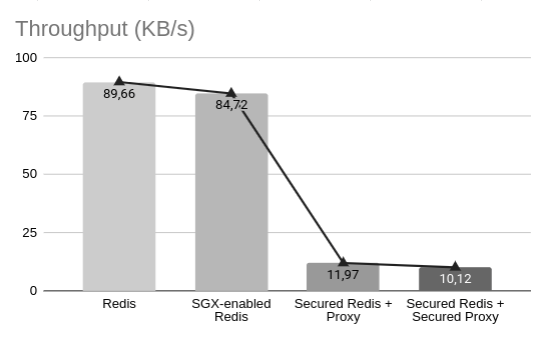
\includegraphics[width=0.7\linewidth]{graphThroughputCluster}}
	\caption{Throughput impact of SGX in Clustered Redis}
	\label{fig:graphTroughputCluster}
\end{figure}

\vspace{40mm}

As for different sets of operations performed over the cluster, the solution shows to also handle them evenly, as it is noted in Table \ref{table:thptDiffRatiosClusterRedis}.

\begin{table}[ht]
	\caption{Throughput with different sets of operations} % title of Table
	\centering % used for centering table
	\begin{tabular}{c c} % centered columns (4 columns)
		\hline\hline %inserts double horizontal lines
		\textbf{Op. Ratio (R:W)} & \textbf{Throughput} \\ [0.3ex] % inserts table
		%heading
		\hline
		1R : 0W & 10,8KB/s\\
		\hline
		10R : 1W & 10,12KB/s \\
		\hline
		1R : 1W & 10,93KB/s\\
		\hline % inserts single horizontal line
		1R : 10W & 10,52KB/s\\
		\hline 
		0R : 1W & 10,8KB/s\\ [0.3ex] % [1ex] adds vertical space
		\hline %inserts single line
	\end{tabular}
	\label{table:thptDiffRatiosClusterRedis} % is used to refer this table in the text
\end{table}

By comparing this values to the ones presented for the previous two configurations, Standalone and Master-Slave, we can conclude that using our solution in cluster mode does not induce in major overheads. Further more, in cluster the solution offers better results while dealing with bigger size requests, as shown in Figure \ref{table:throughputPayloadsCluster}. All this while also offering better availability, scalability and replication of data, along with other properties, than the previously tested configurations.

\begin{table}[ht]
	\caption{Throughput differences with different size payloads} % title of Table
	\centering % used for centering table
	\begin{tabular}{c c c } % centered columns (4 columns)
		\hline\hline %inserts double horizontal lines
		\textbf{Payload Size} & \textbf{Operations p/sec} & \textbf{Latency}\\ [0.5ex] % inserts table
		%heading
		\hline
		10B & $\approx$23 & $\approx$43ms\\
		\hline
		10KB & $\approx$22 & $\approx$44ms\\
		\hline % inserts single horizontal line
		100KB & $\approx$18 & $\approx$54ms\\ [1ex] % [1ex] adds vertical space
		\hline %inserts single line
	\end{tabular}
	\label{table:throughputPayloadsCluster} % is used to refer this table in the text
\end{table} 




\subsection{Clustered REDIS System Resources}

In order to evaluate our Clustered solution's use of resources, we will register the cloud system's behavior while handling 1 KBytes size requests for a duration of 180 seconds.

\begin{figure}[htbp]
	\centering
	{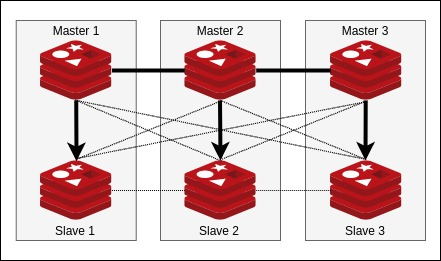
\includegraphics[width=0.5\linewidth]{clusterEvaluation}}
	\caption{Cluster configuration during evaluation}
	\label{fig:clusterLayout}
\end{figure} 

Upon starting the cluster, the Redis instances rearrange themselves to a configuration based on the one shown in Figure \ref{fig:clusterLayout}, with multiple sets combining a master node and one or more slaves. Then, each master node becomes responsible for a set interval of values, that will be used to forward requests upon arrival, based on the request's hash value. Thus, the cluster balances the load between master nodes, which will eventually propagate their data to their respective set of slaves, replicating it.
 
With the cluster assembled according to the model discussed just now, we proceed to register and evaluate the system memory and CPU usage, for both \gls{sgx}-enabled and not.

\begin{figure}[htbp]
	\centering
	\subbottom[) Master 1]{%
		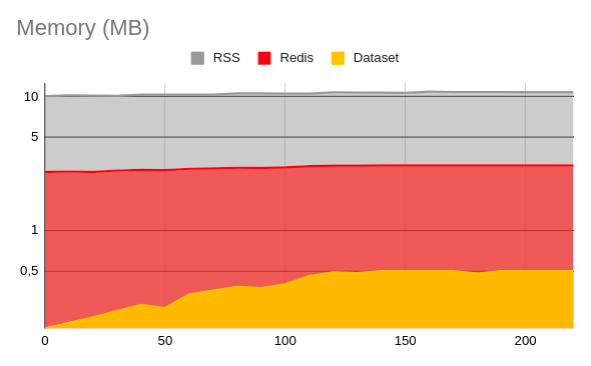
\includegraphics[width=0.4\linewidth]{memoryCluster_M1_noSGX}}%
	\subbottom[) Slave 1]{
		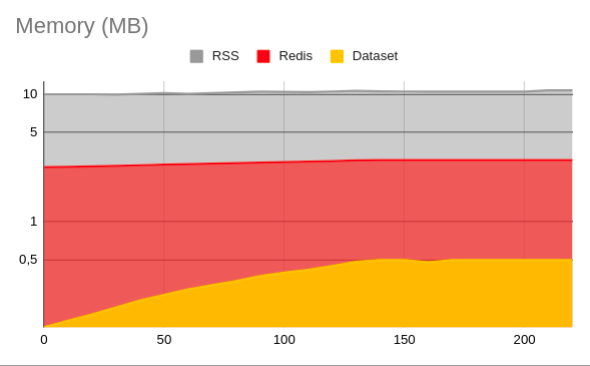
\includegraphics[width=0.4\linewidth]{memoryCluster_S1_noSGX}}
	\subbottom[) Master 2]{
		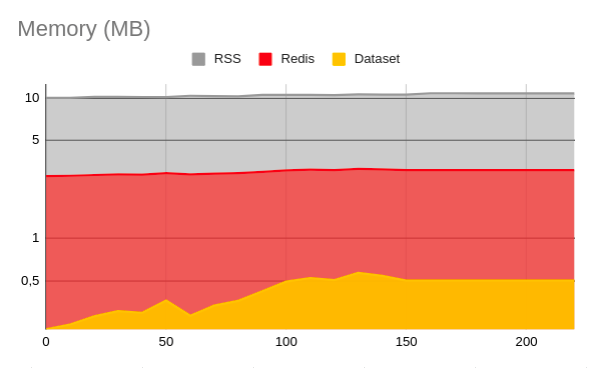
\includegraphics[width=0.4\linewidth]{memoryCluster_M2_noSGX}}
	\subbottom[) Slave 2]{
		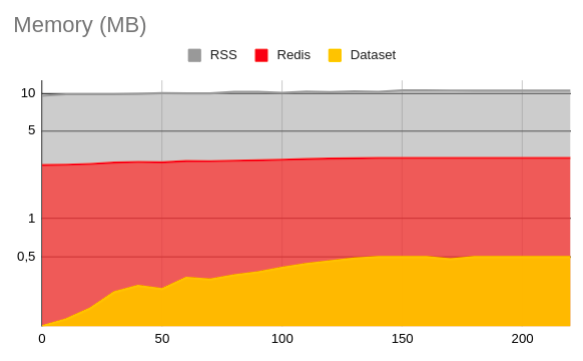
\includegraphics[width=0.4\linewidth]{memoryCluster_S2_noSGX}}
	\subbottom[) Master 3]{
		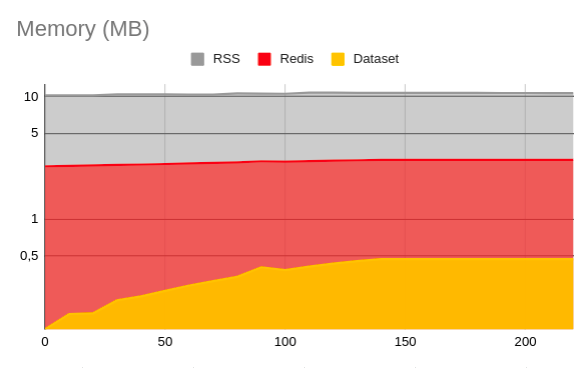
\includegraphics[width=0.4\linewidth]{memoryCluster_M3_noSGX}}
	\subbottom[) Slave 3]{
		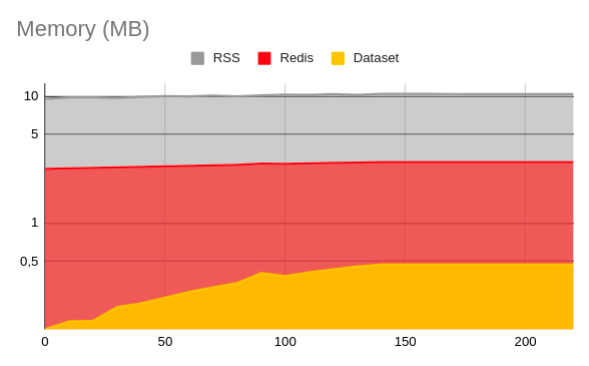
\includegraphics[width=0.4\linewidth]{memoryCluster_S3_noSGX}}
	\caption{Redis Cluster memory consumption}
	\label{fig:noSgxMemoryConsumption_Cluster}
\end{figure}

Starting with the analysis of the solution without \gls{sgx} support, we observe throughput values in the order of $\approx$27 operations per second, which results in a total of around 1500 KBytes writen into the system. By following the cluster design, we see in Figure \ref{fig:noSgxMemoryConsumption_Cluster} that the data is splitted between the master nodes, whereas in the right side graphs, we can see that the slaves end up being replicated by their masters, thus achieving consistency. 

When running our solution in a \gls{sgx}-enabled environment, we achieve results of around 22 operations per second, thus resulting in a slightly smaller Dataset size of $\approx$1300 KBytes. In Figure \ref{fig:sgxMemoryConsumption_Cluster} we see that exact same behavior, with the partitioning of the data taking place between the master nodes, while propagating those partitions to their slave. 
However, and as we have seen in \ref{ssec:SingleRedis_MemCPU} and \ref{ssec:MSRedis_MemCPU}, the RSS value remains static throughout the evaluation. 
Comparing both scenarios where we run the cluster outside \gls{sgx} and inside it, we see a difference of $\approx$75\% more memory allocated by the system for two identical Dataset sizes. Although this memory limit can be manually changed upon starting the instances, this limitation usually results in allocating more memory than what is necessary, in order to prevent the \gls{kvs} instances to run out of memory, and thus stop working.

\vspace{5mm}

\begin{figure}[htbp]
	\centering
	\subbottom[) Master 1]{%
		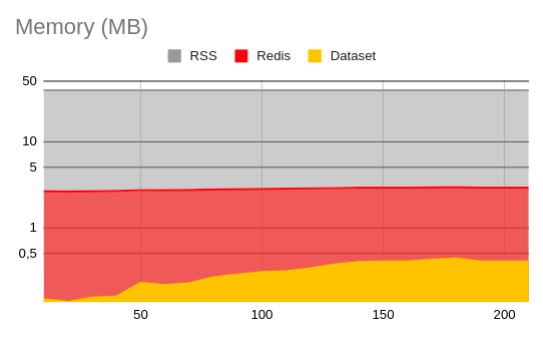
\includegraphics[width=0.4\linewidth]{memoryCluster_M1_SGX}}%
	\subbottom[) Slave 1]{
		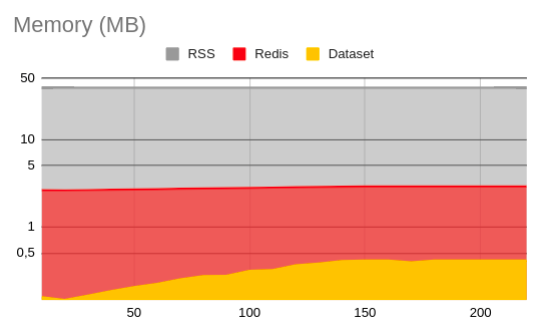
\includegraphics[width=0.4\linewidth]{memoryCluster_S1_SGX}}
	\subbottom[) Master 2]{
		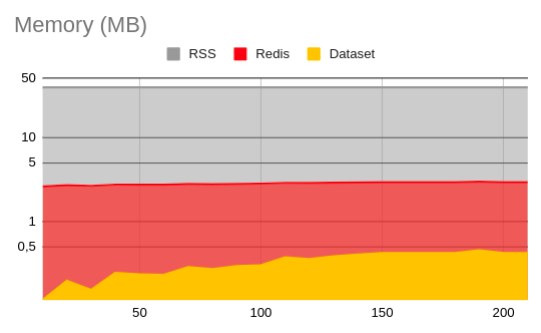
\includegraphics[width=0.4\linewidth]{memoryCluster_M2_SGX}}
	\subbottom[) Slave 2]{
		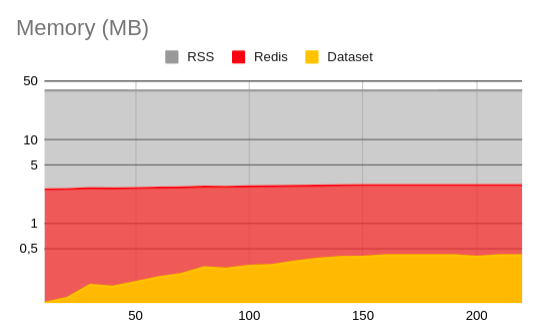
\includegraphics[width=0.4\linewidth]{memoryCluster_S2_SGX}}
	\subbottom[) Master 3]{
		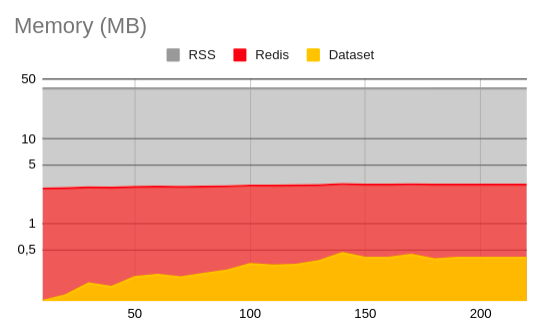
\includegraphics[width=0.4\linewidth]{memoryCluster_M3_SGX}}
		\subbottom[) Slave 3]{
		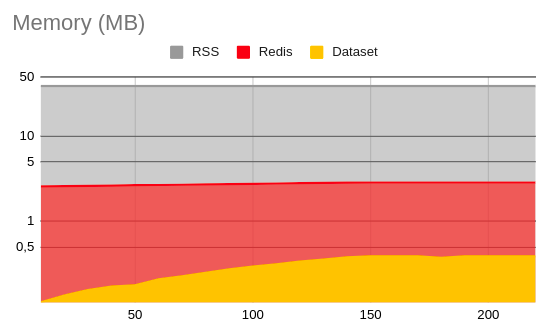
\includegraphics[width=0.4\linewidth]{memoryCluster_S3_SGX}}
	\caption{SGX-enabled Redis Cluster memory consumption}
	\label{fig:sgxMemoryConsumption_Cluster}
\end{figure}

Lastly, Figure \ref{fig:cpuUsageCluster} shows the CPU work that goes into the execution of our solution, either inside or outside a trusted execution environment. 

Here we see that nearly 0\% of the system's CPU resources go into the execution of the Redis instances while running without \gls{sgx} support. However, this value rises to nearly 10\% in the second graph \ref{fig:sgxCPUusageCluster}. This increased value is due to the extra overhead \gls{sgx} gives to the system, along with the data replication among replicas in the cluster.

\begin{figure}[htbp]
	\centering
	\subbottom[) no SGX]{%
		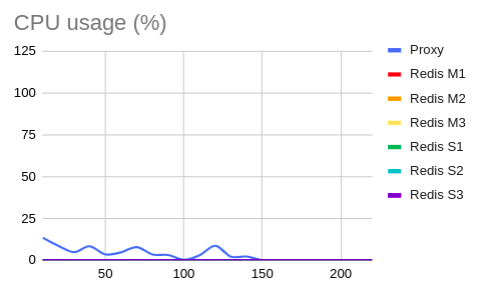
\includegraphics[width=0.51\linewidth]{cpuUsageCluster_noSGX}}%
	\subbottom[) with SGX]{
		\label{fig:sgxCPUusageCluster}
		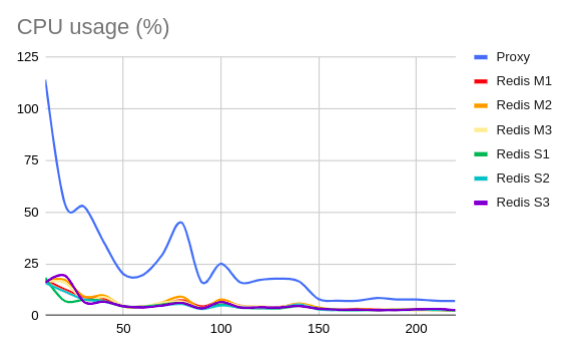
\includegraphics[width=0.51\linewidth]{cpuUsageCluster}}
	\caption{M-S Redis CPU usage during runtime}
	\label{fig:cpuUsageCluster}
\end{figure}

As for the Proxy, its behavior is identical to the previous tests, where we see it going from $\approx$5-10\% to more expressive values when running on top of Intel-\gls{sgx} hardware.

\section{Attestation Impact}

In order to measure the attestation impact in our components, we comply to the scenario described for TB5 defined earlier in \ref{sec:testBenchEnvironments}, where we add the functionality for the \gls{sgx}-enabled components to attest themselves and prove that they are indeed running on private memory regions on top of Intel-\gls{sgx}. 

To assure attestation to our components, we use the mechanism provided by SCONE, consisting in defining secrets to applications on a remote component CAS, where a validation is performed upon starting with the help of a local attestation component LAS. Note that we detailed this process in \ref{ssec:TREDIS_impl_components}. 
We define secrets to be pairs of TLS keys and certificates that applications need upon start to establish TLS connections with other components. Therefore, if an enclave fails to attest itself, it will not have these secrets, thus failing to establish TLS connections, and not starting. These secrets are defined in a YAML file like the one we show in Appendix \ref{app:appendix2}, and sent to a public instance of CAS. 

Our solution's attestation mechanism only allows the SCONE components to be attested upon start and not on-demand. Thus we compare the time it takes a component running in a SCONE container to boot with attestation, comparing it to the time it takes to boot without it. In Table \ref{table:attestationImpactBoot} we observe just that, where we conclude that adding this attestation mechanism to a Redis instance container induce in a $\approx$ 1,23 extra seconds, while for the Proxy $\approx$ 1,05 seconds.

\begin{table}[ht]
	\caption{Attestation impact in boot time} % title of Table
	\centering % used for centering table
	\begin{tabular}{c c c} % centered columns (4 columns)
		\hline\hline %inserts double horizontal lines
		\textbf{} & \textbf{No Attestation} & \textbf{Attestation} \\ [0.5ex] % inserts table
		%heading
		\hline
		\textbf{Redis} & 0,14s & 1,37s\\
		\hline % inserts single horizontal line
		\textbf{Proxy} & 62,07s & 63,12\\ [1ex] % [1ex] adds vertical space
		\hline %inserts single line
	\end{tabular}
	\label{table:attestationImpactBoot} % is used to refer this table in the text
\end{table}

\section{Main Findings From the Experimental Observations}

During the evaluation in this chapter, we were able to analize our solution in three different configurations, Standalone, Master-Slave and Cluster, by following multiple testbenches that were previously described, in order to benchmark the impact that securing our solution's components with \gls{sgx} has overall. 

After going through all the results for each configuration, we see that although the system has lost some performance with the addition of \gls{sgx}, its impact can be looked at as quite modest, varying from low to medium on all components involved in the evaluation, regardless the mode the \gls{kvs} is set to execute. 

However, after comparing the different evaluations made over the three Redis configurations, we see slightly better performance results in the last one, performed over a Clustered Redis. Adding to that, by being a cluster, it offers extra properties to the system itself, like partitioning and replication of data, availability, scalability, and so on, which helps us think that the Cluster mode is the more suitable Redis configuration to be used in a \gls{sgx}-enabled environment.

As for the Proxy, since our intention is to recreate a real-world scenario where the TREDIS can be used as a normal application in cloud, it is essencial that our solution is enabled to receive requests via HTTP. Thus, the $\approx$80\% impact it has on the performance caused by adding the Proxy alone as to be taken as a necessity and not as the drop itself. However, there is room here for improvement, since our Proxy was designed in Java, which led to more code being needed. 

\section{Summary}

In this chapter, we evaluated the solution we proposed for this dissertation, an in-memory TREDIS solution, introduced in Chapter \ref{cha:systemModel_and_design} and detailed in Chapter \ref{cha:implementation}. Here we conducted a study about the impact that \gls{sgx} has in the components that make up our solution, in order to analyse if the tradeoff between performance and security is worth it or not. 

To access its impact, we benchmarked the solution according to defined testbenches, each one representing a different scenario, that we used to perform a structured incremental analisis where we added system components one by one, while also adding security to them one by one, starting with the Redis layer unprotected and gradually building up to the point we had the whole solution running on top of \gls{sgx}. We also defined some extra testbenches in order to evaluate other more specific measurements. All the testbenches were repeated for the three Redis configurations we mentioned, Standalone, Master-Slave and Cluster, in order to see their behavior running in a \gls{sgx}-enabled environment.

During the evaluation, we concluded that while the overall tendency of using Intel-\gls{sgx} results in overheads, the values go from having low to medium impact overall, never going past 18\%. 

The biggest impact to our solution comes from the Proxy component, whether by enabling it to \gls{sgx} support or by its inclusion in the solution itself. However, we found this component to be essential for our solution to work as we intend, not only because of the purposes we assigned to it, which are described in \ref{ssec:sgx_redisSolution}, but also because it makes our solution more practical in real-world scenarios, working as an API that can be exposed to clients that they can reach through the web, via HTTP.

